\documentclass[a4paper]{article}
\usepackage[top=30pt,bottom=30pt,left=48pt,right=46pt]{geometry}

\usepackage[utf8]{inputenc}			% accents
\usepackage[T1]{fontenc}			% accents et césure
\usepackage{lmodern}				% image vectorielle
\usepackage{graphicx}
\usepackage[english]{babel}
\usepackage{physics}
\usepackage{amsmath}
\usepackage{amssymb}
\usepackage{mathrsfs}

\begin{document}

\title{Brunel Network}
\author{Bruno Magalhaes, Gael Reganha, Leo Sumi, Thais Lindemann, Johannes Brune, Laure Font,\\ Laurine Kolly, Violette Zanotti, Julie Brancato, Fiona Joseph, Clara David-Vaudey}
\maketitle

\paragraph{Model}

The Leaky integrate-and-fire (IF) neuron model is described as an electrical model of a neuron with a resistance R and capacity C:
\begin{equation}
  \tau \frac{dV}{dt}(t) = -V(t) + RI(t) \text{ with } \tau = R C 
  \label{equation_diff}
\end{equation}
where $RI(t)$ is the network contribution:
\begin{equation}
   RI(t) = \tau \sum_{i} J_{ij} \sum_{t^\prime} \delta (t-t^\prime _{j} -D)
  \label{equation_current}
\end{equation}
where $J_{ij}$ is the postsynaptic potential amplitude, 
$\delta (t)$ the dirac function, $t^\prime _{j}$ the spiking time of pre-synaptic neuron $j$ at time $t^\prime$ and 
$D$ the transmission delay. For simplicity we represent $V(t)$ as $V_t$. \\

\paragraph{Analytical solution}

We consider that the neuron is able to steeply rise its potential when there is an input of current, thus discarding the exponential charge of the capacitance. The discharge follows an exponential decay with the time constant $\tau$. We compute two different stepping methods from the analytical solution: 
\begin{itemize}
\item \textbf{Two step algorithm}:
\begin{enumerate}
  \item Calculate decay from previous step: $V_t \leftarrow V_{t- \Delta t} exp(\frac{-dt}{\tau})$  
  \item Add voltage change of network current $RI$ between $t-\Delta t$ and $t$: $V_t \leftarrow  V_t + RI_{(t-\Delta t, t]} / \tau $
  \end{enumerate}
\item \textbf{fixed step} interpolation assumes $\Delta t$ to be constant throughout the execution. The \textbf{Variable step} method advances the neuron with the smallest $t$ on the network, with a $\Delta t$ computed as the minimum of the two following values:
\begin{itemize}
\item the time difference to the next incoming spike;
\item $t^\star + D$ where $t^\star$ is the time of the neuron with the second smallest $t$, i.e. the largest step that can be taken from neuron at $t$ so that it won't miss a spike from neuron at time $t^\star$, if it spikes.  
\end{itemize}
\end{itemize}

\paragraph{Euler methods}

For efficiency purposes, we implemented two approximated fixed-step Euler methods:
\begin{itemize}
\item \textbf{Explicit Forward Euler:} $\tau \frac{dV_{t}}{dt} = -V_{t - \Delta t} + RI_{(t-\Delta t, t]} \Leftrightarrow V_t = V_{t - \Delta t} +  \frac{dV_{t- \Delta t}}{dt} \Delta t \Leftrightarrow  V_t = \frac{-V_{t - \Delta t} + RI_{(t-\Delta t, t]}}{\tau} \Delta t$
\item \textbf{Implicit Backward Euler:} $\tau \frac{dV_{t}}{dt} = -V_{t} + RI_{(t-\Delta t, t]} \Leftrightarrow \frac{V_{t} - V_{t - \Delta t}}{\Delta t} = -V_{t} + RI_{(t-\Delta t, t]} \Leftrightarrow V_t = \frac{RI_{(t-\Delta t, t]} + \tau * V_{t-\Delta t}}{\Delta t + \tau}$
\end{itemize}

with $\frac{dV_{t}}{dt}$ and $RI_{(t-\Delta t, t]}$ computed from equations \ref{equation_diff} and \ref{equation_current} respectively\footnote{$RI_{(t-\Delta t, t]}$ is divided by $\Delta t$ so that it is expressed in voltage per time-unit instead of per time-step.}.

\paragraph{Results} We present the potential over time of neuron $0$ for the aforementioned methods on a $100ms$ simulation of a Brunel network of $10000$ neurons with random seed $0$ and default neuron parameters:

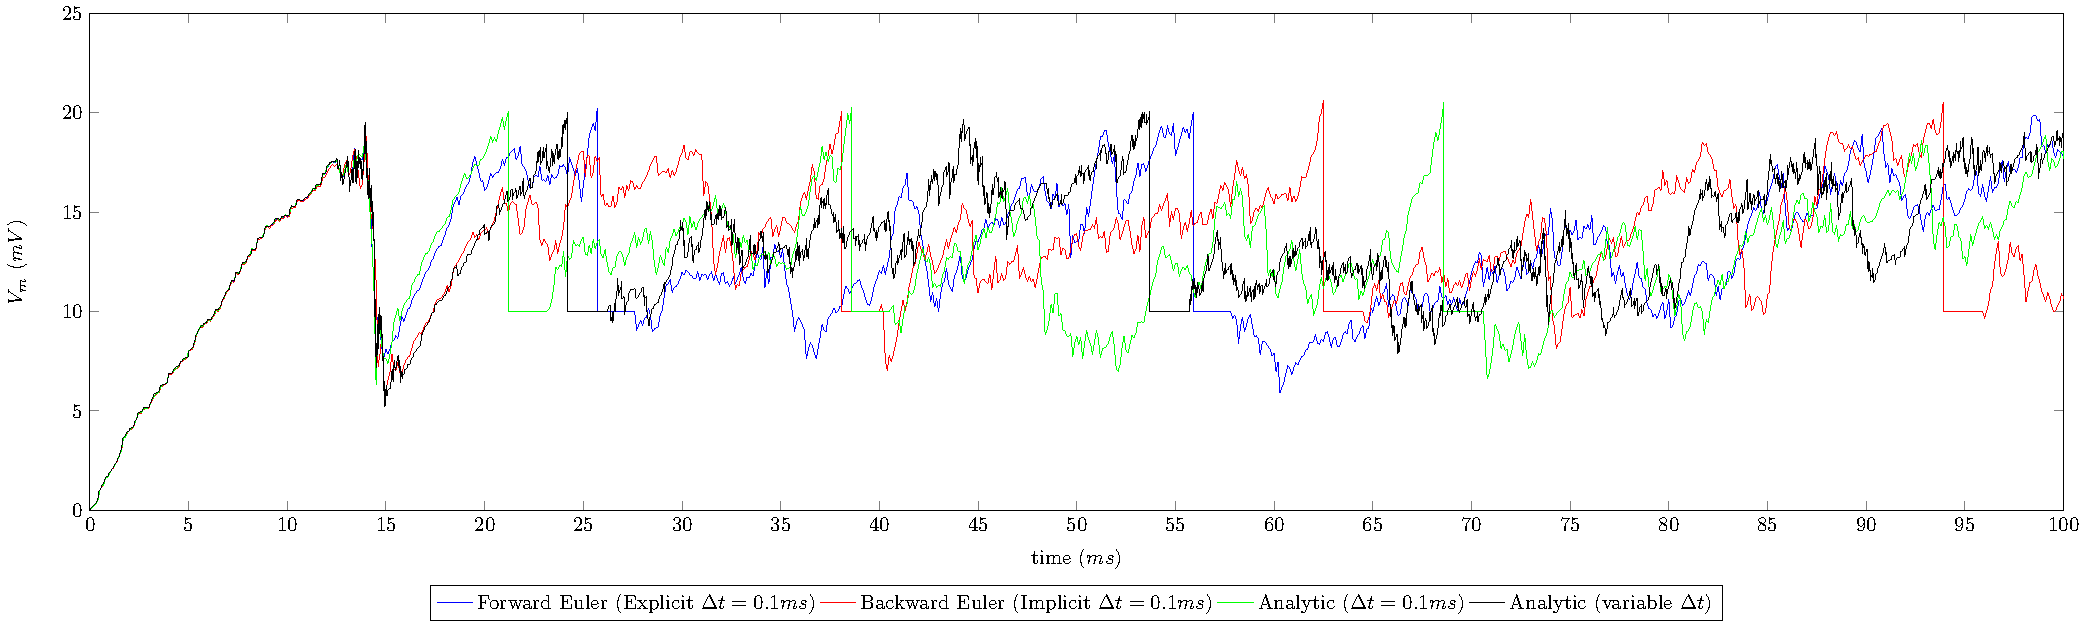
\includegraphics[width=1.0\textwidth]{./neuron_plot_equations.pdf}

%\includegraphics[width=1.0\textwidth]{./raster_plot_analytic_fixed_step.pdf}


\end{document}
